\chapter{Level Set Methods}
\newcommand{\uxt}{$u(\mathbf{x}, t)$ }

A level set formulation is an implicit representation of a closed curve or curves. 
The curve is represented as a constant value of a higher dimensional function.
A familiar example of such level curves are level curves on a map. Provided 
a continuous function of the elevation of the ground surface on an area, the level
contours joins points on the surface of equal elevation. All curves representing the 
same value, or elevation in the cartographic setting, are called \textit{iso-curves} or
\textit{iso-contours}. On a map, there are numerous iso-curves of different values 
separated by a constant height. Such contours are thus effectively describing
the steepness and height, and thus the shape, of the ground in the area. 
In a level set context, we are not interested in the shape of the underlying 
higher dimensional function. We look at a single iso-value and the standard 
practice is to use the zero iso-value. The corresponding curve(s) will 
split the domain into regions of two types. One where the underlying function is 
positive, and one where it is negative. In contrast to cartography, level set 
methods only tracks the shape of the surfaces of these regions and how they 
change over time.

\todo{cool: image of a function that is cut at a specific value}

\begin{comment}
To continue with the cartographic image, 
The image of contours on a map is useful when understanding iso-curves in a
level set setting also. Since the level set formulation is a way of describing
closed curves, we need to know under which circumstances iso-contours forms 
closed curves. As we are used to from maps, elevation curves are always closed.
\todo{Fullfør. Kontinuitet?}
\end{comment}

\section{Level Set Definition}
Now that we have an intuition about iso-curves, we can discuss the principle
of a level set method. The goal is to represent a closed curve or surface, 
$\Gamma(t)$, that moves under the influence of a velocity field $\vv{v}$.
The level set approach to this problem, as first presented in 1987 by 
S.Osher and J. Sethian \cite{MR965860}, is to define a continuous function
\uxt defined on a domain $\mathcal{D}$ containing $\Gamma|_{t=0}$.
The domain $\mathcal{D}$ is split in two parts by the curve $\Gamma$, the interior
$\Omega$ and the exterior $\mathcal{D} \setminus \Omega$. 
\begin{figure}
    \centering
    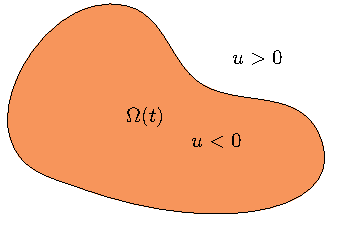
\includegraphics[width=.5\linewidth]{figures/tikz-figures/optimization-problem.pdf}
    \caption{Level set representation of a curve $\Gamma (t)$.}
    \label{fig:levelset-representation}
\end{figure}
The function \uxt must be constructed in a way that it satisfies the following properties
\begin{align}
    u(\mathbf{x}, t) < 0 \qquad &\text{for } \mathbf{x} \in  \Omega(t) \label{eq:interior}\\
    u(\mathbf{x}, t) = 0 \qquad &\text{for } \mathbf{x} \in  \Gamma(t) \label{eq:zero-iso-curve}\\
    u(\mathbf{x}, t) > 0 \qquad &\text{for } \mathbf{x} \in  \mathcal{D} \setminus \Omega(t) \label{eq:exterior}.
\end{align}
Now, the curve $\Gamma$ can be described in terms of \uxt by being its 
zero iso-contour. This means that if we can find the proper evolution of 
\uxt we can implicitly track the motion of the curve $\Gamma$.
What we now want is to find the right motion for \uxt to
track the level curve $\Gamma$ flowing in the velocity field $\vv{v}$. Because
we are only interested in the movement of the zero iso-curve of \uxt,
differentiate \eqref{eq:zero-iso-curve} with respect to time to find the movement
of $\Gamma$ when \uxt changes.
\begin{equation}
    (u(\mathbf{x}, t)_t + \nabla u(\mathbf{x}, t) \, \Gamma_t)_{\mathbf{x}\in \Gamma} = 0
    \label{eq:general-u-flow}
\end{equation}
When $\Gamma$ flows in the velocity field $\vv{v}$, its time derivative has to be 
defined as \todo{dette er ikke helt bra:}
\begin{equation}
    \Gamma_t = \vv{v}\cdot \vv{n}_{\Gamma} = v_n \vv{n}_{\Gamma}.
\end{equation}
In addition, we can see from \eqref{eq:interior}-\eqref{eq:exterior} that the gradient 
of $u$ at the curve $\Gamma$ is always pointing in the direction of the normal vector of 
$\Gamma$, $\vv{n}_{\Gamma}$. Thus we can write 
\begin{equation}
    \vv{n}_{\Gamma} = -\frac{\nabla u}{|\nabla u|}
\end{equation}

Inserting everything back into \eqref{eq:general-u-flow}, we get the equation
\begin{equation}
    u_t - v_n\, |\nabla u| = 0
    \label{eq:general-level-set}
\end{equation}

Now we have derived a PDE that will move surface or a curve under the influence
of a velocity field $\vv{v}$. However, there exists other methods to model
a moving surface and thus we ask the question: How does the level set 
formulation differ from other methods and in what situations could this be 
a preferred choice?




What to discuss around the method?
\begin{enumerate}
    \item increased complexity for solving PDE on entire domain. How to fix
    \item Topological flexibility. Situations that are now easily handled.
    \item Existence of viscosity solution (?????). In that case, I must read.
    \item Existence and uniqueness
\end{enumerate}

\newpage
\section{Gradient flow}
We now want to use a level set method to solve a problem as described in the
introduction. We have sampled data from an unknown surface/curve and want to
reconstruct the original surface. We then want to find the appropriate velocity
field from \eqref{eq:general-level-set} in a way such that our surface $\Gamma$ 
flows in the direction of our points at the same time as it preserves smoothness. We
approach this by formulating the situation as an optimisation problem, or more
specifically, we construct a \textit{gradient flow equation} for our domain $\Omega$. 

Gradient flow is the continuous version of the steepest descent algorithm. The descent methods are optimisation algorithms for finding minimisers of functionals and the idea is
to always move in the direction of steepest descent. Mathematically this is formulated as follows. \todo{define variables} 
\begin{equation}
    X_t = -\nabla f(X).
\end{equation}

In order to use this optimisation formulation, we need to construct a function depending
on the domain $\Omega$ that has a minima when, $\Gamma$, the surface of $\Omega$
is the desired surface we are looking for. As we are introducing the movement of $\Gamma$
as a flow, it fits nicely to call this function we are optimising, an energy function. 
Using that, we can think of our curve moving in a type of gravitational field, drawn
towards the point set V and influenced by a surface tension to ensure smoothness. 

The energy function is only a tool to ensure that the surface, $\Gamma$, flows towards the
desired stationary solution, so the function could be described in numerous ways as long 
as a minima is obtained at our desired curve. However, some functions are more fit than others, as we want hopefully the global minima at the curve and ...    

We would like to move the curve, which is equivalent to changing the interior 
$\Omega$ , such that we minimise the energy functionals defined above \todo{Ikke gjort}. 

* Minimise the functionals we find above. 

* Define our new PDE with the new velocity field. Discuss terms and parameters.

* Local and global minima of the optimisation problem. Integral over domain = Ø is zero. To have a global min on the curve, we need the interior to be negative.

* From the optimisation formulation, we will find the minima which will
be equivalent to finding the stationary solution for our curve. NB: This could not be
the global stationary solution. The velocity will be zero only on the curve. Thus 
we need a stopping criterion for the problem \eqref{eq:general-level-set}. 

\section{Existence of a stationary solution}

